% !TEX root = ../Dokumentation.tex
\newpage
\subsection{Chassis}
\textbf{Funktionsbeschrieb}\\[0.2cm]
Bei der Umsetzung wird ein Chassis mit vier Rädern verwendet. Die Hinterräder werden mit einem DC-Motor mit Encoder angetrieben. Der Motor ist über ein Differentialgetriebe mit der Hinterachse verbunden. Das Differentialgetriebe erlaubt den beiden Hinterrädern in der Kurve unterschiedlich schnell zu drehen. Die Vorderräder sind frei drehbar. Der Achsabstand soll ein Mass von 160mm nicht überschreiten.\\
Für die Lenkung wird eine Achsschenkellenkung verwendet. Diese wird mittels eines Servomotors über eine Kegelradverbindung angetrieben. Wegen dem maximalen Achsabstand von 160mm ist der Servomotor zum Antrieb der Lenkung vor dem Fahrzeug verbaut.
\begin{figure}[H]%Position festigen
\centering
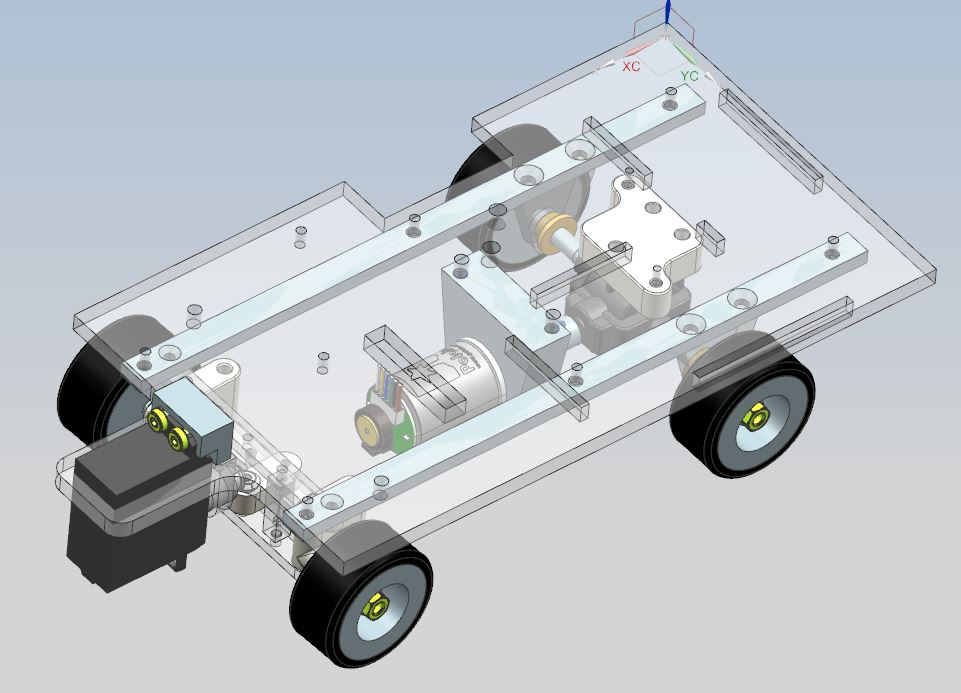
\includegraphics[width=0.8\textwidth]{03_Loesungskonzept/pictures2/Chassis.JPG}
\caption{Chassis}
\label{fig:activityRoute}
\end{figure}
\newpage
\textbf{Komponenten}\\[0.2cm]
\begin{figure}[H]%Position festigen
\centering
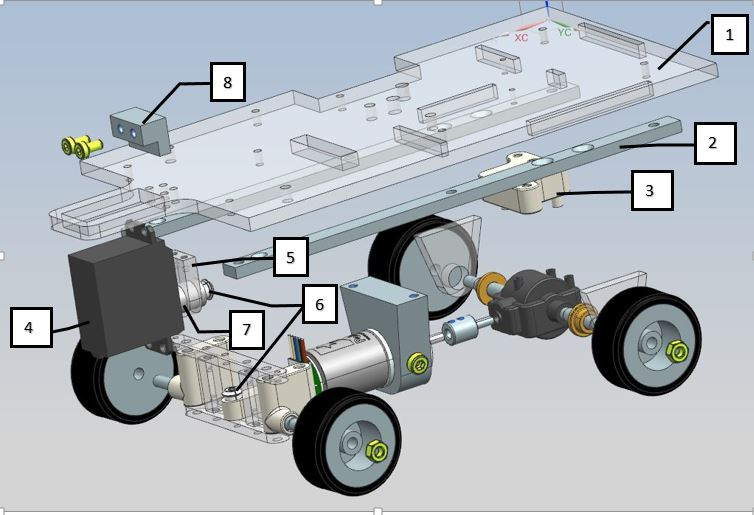
\includegraphics[width=0.8\textwidth]{03_Loesungskonzept/pictures2/Explosion_Chassis_1_lg.JPG}
\caption{Chassis mit Komponentenbeschriftung 1}
\label{fig:activityRoute}
\end{figure}
\begin{figure}[H]%Position festigen
\centering
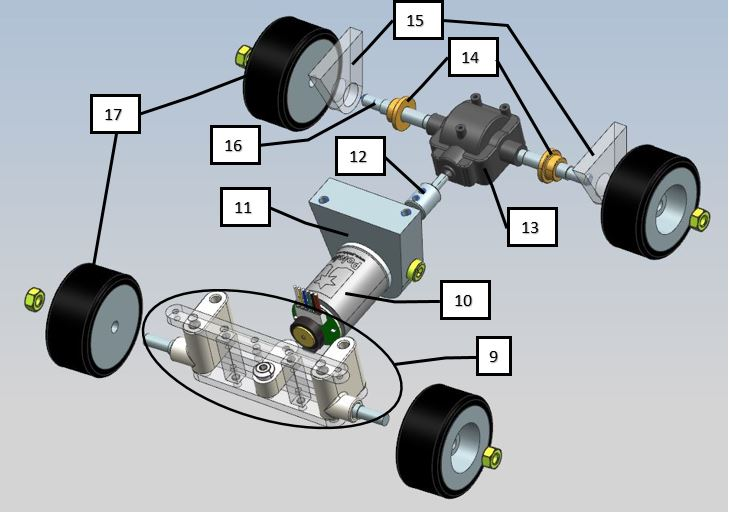
\includegraphics[width=0.8\textwidth]{03_Loesungskonzept/pictures2/Explosion_Chassis_2_lg.JPG}
\caption{Chassis mit Komponentenbeschriftung 2}
\label{fig:activityRoute}
\end{figure}
\newpage
\textbf{Positionsnummernbeschrieb}\\[0.2cm]
Pos.1 	Grundplatte\\
Pos.2 	Stützstreben\\
Pos.3 	Halterung für Differenzial\\
Pos.4 	Servomotor Lenkung\\
Pos.5 	Halterung für Kegelrad\\
Pos.6 	Kegelrad m=0.5, i=1, z=16\\
Pos.7 	Verbindung Servomotor und Kegelrad\\
Pos.8	Haltewinkel Lenkservo\\
Pos.9	Achsschenkellenkung (Komponentenbeschrieb im Kp 2.3 Lenkung)\\
Pos.10	Ponolulu DC-Motor mit Encoder\\
Pos.11	Halter für DC-Motor\\
Pos.12	Verbindung DC-Motor Differential\\
Pos.13	Differentialgetriebe von Modellbauhersteller Relly\\
Pos.14	Bundbuchsen aus Sinterbronze, Form V ähnlich DIN 1850\\
Pos.15	Achsaufhängung hinten\\
Pos.16	Hinterachsen\\
Pos.17	Räder von Legobausatz D43.3cm\\[0.2cm]
\textbf{Fertigung, Beschaffung und Material}\\[0.2cm]
Pos.1 	Laserschneiden HSLU / Acrylgras 6mm\\
Pos.2 	Werkstadtfertigung HSLU / AlMgSi1 Profil 5x10mm\\
Pos.3 	3D-Druck HSLU\\
Pos.4 	Bezogen über HSLU\\
Pos.5 	Laserschneiden HSLU / Acrylgras 6mm\\
Pos.6 	Bestellt bei Mädler / Kegelräder aus Azetalharz\\
Pos.7 	Werkstadtfertigung HSLU / AlMgSi1\\
Pos.8	Werkstadtfertigung HSLU / AlMgSi1\\
Pos.9 	Siehe Kp 2.3 Lenkung
Pos.10	Bestellt von Ponolulu (nähere Beschreibung Kap 2.4 Antrieb\\
Pos.11	Werkstadtfertigung HSLU / AlMgSi1\\
Pos.12	Werkstadtfertigung HSLU / AlMgSi1\\
Pos.13	Bestellt bei Conrad / Kunststoff\\
Pos.14	Bestellt bein Mädler / Sinterbronze\\
Pos.15	Laserschneiden HSLU / Acrylglas 6mm\\
Pos.16	Werkstadtfertigung HSLU / S235JRG2C\\
Pos.17	Zur Verfügung gestellt von Teammitglied / Kunststoff\\[0.2cm]
Bemerkung: Alle Fertigungszeichnungen sowie Bestelllisten für Dritthersteller, 3D-Druckteile und Laserteile sind im Anhang.\\
\textbf{Schwierigkeiten}\\[0.2cm]
Bei der Montage hat sich herausgestellt, dass das Montieren der Hinterachsen mit auf einer Linie mit den Gleitlagerbuchsen und dem Differentialgetriebe sich als schwierig gestaltet. Da die Halterung für das Differentialgetriebe ein 3D-Druckteil ist, war die Fertigungsgenauigkeit nicht hoch genug. Dies hatte zu Folge, dass das Differentialgetriebe nicht genau auf einer Flucht mit der Achsaufhängung war. Um dieses Problem zu beheben, mussten wir die Schraubenlöcher der Halterung aufbohren um mehr das Differential leicht zu verschieben.\\
Ein weiteres Problem war die Befestigung der Hinterachsen im Differentialgetriebe. Da nicht alles genau auf einer Flucht ist, gibt es beim Fahren leichte exzentrische Bewegungen der Achsen. Durch diese Bewegungen löste sich der zur Befestigung verwendete Zweikomponentenleim und die Achsen drehten nicht mehr mit. Um sicherzustellen, dass die Achsen auf jeden Fall mitdrehen und sich nicht lösen, wurde ein kleines Loch (D 1mm) durch Achse und Differentialgetriebe gebohrt. Durch dieses Loch wurde dann ein Draht gefädelt.\\[0.2cm] 
\textbf{Änderungen zum Konzept aus PREN1}\\[0.2cm]
Um das entwerfen und Bauen eines eigenen Encoders zu ersparen, wurde der Motor vom ursprünglichen DC-Getriebemotor ohne Encoder zu einem DC-Motor mit eingebautem Encoder der Firma Ponolulu gewechselt. Weitere Informationen im Kp 2.4 Antrieb.
